\section{Introdução e Justificativa}
\label{sec:int}

Os avanços na tecnologia estão permitindo que as pessoas utilizem de serviços com um grande volume de dados. Essa onda, atualmente conhecida como BigData, tem atraído pesquisadores para testar e validar novas abordagens devido ao grande desenvolvimento de aplicações distribuídas \cite{mmo_analytic}.

Um dos temas abordados são os serviços de jogos de interpretação multijogador massivos (popularmente conhecidos por MMORPG, ou \textit{Massively Multiplayer Online}), estes que surgiram de uma categoria de jogos de mesa baseados em representação de personagens nomeado como \textit{Role-Playing Game} (RPG) tal como o jogo \textit{Dungeon and Dragons} \cite{tsr1980dungeons}. A principal característica desse estilo de jogo é a comunicação e representação virtual de um mundo onde cada jogador pode interagir com objetos virtuais compartilhados ou tomar ações sobre outros milhares de jogadores, tendo como maior objetivo do jogo a resolução de problemas, desenvolvimento do personagem e interação entre os jogadores \cite{video_game_technologies}.

O mercado de jogos massivos vem crescendo desde 2012 \cite{new_york_times}, sendo 2016 um dos mais lucrativos até então segundo o site Statista \cite{statista_2016}. A sua projeção para 2018 é que sejam arrecadados mais de 30 bilhões de dólares americanos com esta categoria de jogos \cite{statista_2018}, um aumento de 20\% a mais sobre o ano de 2016.

Um estudo realizado \cite{system_performance} mostra um serviço de MMORPG utilizando 4 servidores distintos separados por um multiplexador. Pode-se perceber que existem picos próximos a 2250 conexões simultâneas ~\ref{fig:conection_peer_hour}, mesmo o jogo analisado sendo considerado um jogo de pequeno porte. Jogos de porte maior podem conter milhares de jogadores online simultaneamente. Um exemplo é o jogo entitulado RuneScape, a qual possui 90 mil jogadores online simultaneamente \cite{runescape_online_users}, mostrando assim a carga que a carga que serviços como esses devem suportar.

\begin{figure}[h]
  \caption{Plot gráfico comparando o número de conexões ao decorrer de 11 dias
  \cite{system_performance}.}
  \centering
  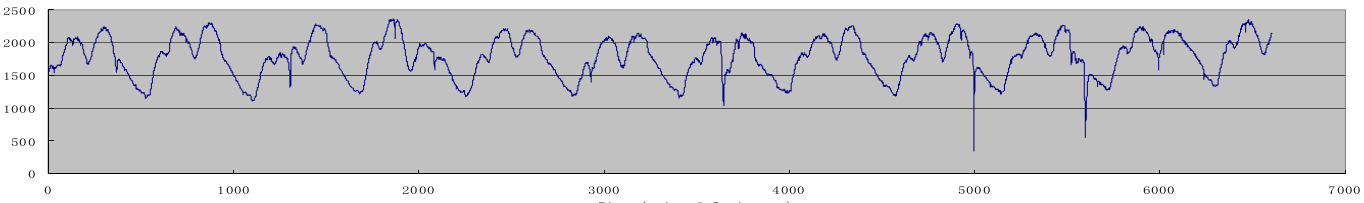
\includegraphics[width=1\textwidth]{img/connection_peer_hour.png}
  \label{fig:conection_peer_hour}
\end{figure}

Em geral, serviços para essa categoria de jogo tendem a tranportar e manipular uma grande quantia de dados, e por esse motivo torna-se alvo de diversas pesquisas nas áreas de sistemas distribuidos e redes de computadores com o objetivo de minimizar o impácto da latência nesses serviços\cite{stephenclarkewillson2017} e por sua vez aumentar a qualidade de serviço. Vários estudos focaram em distribuição de carga \cite{load_balance} \cite{kd_tree}, e arquiteturas \textit{peer-to-peer}.

Os serviços atuais escritos para suportar milhares de jogadores atualmente estão trabalhando como microserviços\cite{stephenclarkewillson2017}\cite{albion_online_unite}. Estes microserviços são pequenos softwares que realizam uma determinada ação de forma exemplar, uma evolução do conceito de utilidades Unix "\textit{doing one thing well}". Esses serviços pertencem a uma coleção de serviços denominada macroserviço, a qual corresponde ao serviço completo de backend da aplicação.
